\chapter{Entwurfsmuster}
Entwurfsmuster sind bewährte Methoden, um wiederkehrende Probleme in der Softwareentwicklung zu lösen und stellen somit eine Art Blaupause dar, die zur Verbesserung der Struktur, Klarheit und Flexibilität von Software beitragen. Auch in diesem Projekt wurden Entwurfsmuster eingesetzt. Eines dieser Entwurfsmuster soll im nachfolgenden Abschnitt genauer erläutert werden.

\section{Observer Pattern}
In der Rezept-Anwendung wurde vermehrt mit dem Entwurfsmuster Observer-Pattern (Beobachter) gearbeitet. Das Observer-Entwurfsmuster ermöglicht es, Änderungen an einem Objekt den anderen Objekten mitzuteilen, die sich dafür registriert haben. Der Observer gehört zu der Kategorie der Verhaltensmuster. Das Entwurfsmuster besteht aus zwei Hauptkomponenten: dem Observable (Subjekt) und den Observern (Beobachtern). 
Das Subjekt hat einen Zustand, der sich im Laufe der Zeit ändern kann. Die Beobachter registrieren sich beim Subjekt und werden automatisch benachrichtigt, wenn sich der Zustand des Subjekts ändert. Das Observer-Entwurfsmuster ermöglicht es, Objekte lose zu koppeln, da die Observer keine Kenntnis über den Zustand der Objekte haben müssen, auf die sie reagieren. Dies führt zu einer flexibleren und wartungsfreundlicheren Softwarearchitektur.
Im Folgenden wird das Entwurfsmuster anhand eines Beispiels genauer erläutert. 

In der entwickelten Anwendungen wurde mit Java Swing gearbeitet, welche einen Observer (Beobachter) zur Verfügung stellt. Java Swing wurde genutzt, um die Benutzeroberfläche in der Java Anwendung zu erstellen. Diese Benutzeroberfläche ist interaktiv. Um auf die Benutzerinteraktionen zu reagieren, stellt Java Swing das Interface Action Listener bereit. Der Action Listener ist in unserer Anwendung der konkrete Observer (Beobachter) und der JButton das konkrete Subjekt. 
\begin{figure}[ht]
	\centering
	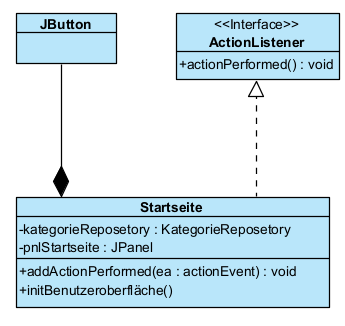
\includegraphics[width=0.50\textwidth]{Bilder/Entwurfsmuster-UML.png} 
	\caption{UML-Diagramm Observer-Pattern Entwurfmuster}
	\label{fig:EntwurfmusterUML}
\end{figure}

Abbildung \ref{fig:EntwurfmusterUML} ist das UML-Diagramm unseres Observers. 
